%%%%%%%%%%%%%%%%%%%%%%%%%%%%%%%%%%%%%%%%%
%
% (c) 2020 by Jennifer Laaser
%
% This work is licensed under the Creative Commons Attribution-NonCommercial-ShareAlike 4.0 International License. To view a copy of this license, visit http://creativecommons.org/licenses/by-nc-sa/4.0/ or send a letter to Creative Commons, PO Box 1866, Mountain View, CA 94042, USA.
%
% The current source for these materials is accessible on Github: https://github.com/jlaaser/pogil-polymers
%
%%%%%%%%%%%%%%%%%%%%%%%%%%%%%%%%%%%%%%%%%

\renewcommand{\figpath}{content/intro/size-and-complexity/figs}
\renewcommand{\labelbase}{size-and-complexity}

\begin{activity}[With Increasing Size Comes Increasing Complexity]

\begin{instructornotes}

	This activity introduces students to key concepts related to the size and molecular weight of polymer molecules, and conformational flexibility.
	
	After completing this activity, students will be able to:
			\begin{enumerate}
				\item Calculate the molecular weight of a polymer, given the number of repeat units and molecular weight of each repeat, and vice versa
				\item Estimate the physical extent of a polymer that is (a) fully extended, (b) fully collapsed, or (c) somewhere inbetween
				\item Estimate the number of conformations available for a polymer molecule
			\end{enumerate}
			
	\subsection*{Activity summary:}
	\begin{itemize}
		\item \textbf{Activity type:} Learning Cycle
		\item \textbf{Content goals:} Introduction to polymers
		\item \textbf{Process goals:} %https://pogil.org/uploads/attachments/cj54b5yts006cklx4hh758htf-process-skills-official-pogil-list-2015-original.pdf
			written communication, critical thinking, information processing
		\item \textbf{Duration:} TBD
		\item \textbf{Instructor preparation required:} none beyond knowledge of relevant content
		\item \textbf{Related textbook chapters:}
			\begin{itemize}
				\item \emph{Polymer Chemistry} (Hiemenz \& Lodge): section 1.2
			\end{itemize}
		%\item \textbf{Facilitation notes:}
		%	\begin{itemize}
		%		\item \dots
		%	\end{itemize}
	\end{itemize}
	
\end{instructornotes}




\begin{model}[Molecular Weight and Degree of Polymerization]
\label{\labelbase:mdl:polyethyleneMW}

	The structure of polyethylene is shown below:

	\vspace{6pt}
	\centerline{\includegraphics[scale=2]{\figpath/Model1_nrepeats.pdf}}
	\vspace{6pt}
	
	The repeat unit has a chemical formula of \ce{C2H4} and a molecular weight of 28 g/mol.

\end{model}


\begin{ctqs}

	\question Consider a molecule of polyethylene with 100 repeat units.  What would the molecular weight of this molecule be?
			
				\emph{Note: for the purposes of this activity, you may ignore the \ce{CH3} end groups on the chain, and only consider the atoms in the repeat units.}
	
		\begin{solution}[1.75in]
		\end{solution}
				
	\question Conversely, consider a molecule of polyethylene with a molecular weight of 700~kg/mol.  Approximately how many repeat units would this chain contain? \label{\labelbase:ctq:700kgPE}
	
		\begin{solution}[1.75in]
		\end{solution}
	
\end{ctqs}

\begin{infobox}

	The number of repeat units in a polymer chain, $N$, is referred to as the \emph{degree of polymerization}.

\end{infobox}

\begin{ctqs}
		
	\question What would the molecular weight of a polyethylene molecule with degree of polymerization $N$ be?
	
		\begin{solution}[1in]
		\end{solution}
		
	\question More generally, suppose a molecule is made up of $N$ repeat units whose molecular weight is $M_0$.  What would the molecular weight of this molecule be?
	
		\begin{solution}[1in]
		\end{solution}
	
	\question Explain, in 1-2 complete sentences, how you could calculate each of the following:
	
		\begin{enumerate}
			\item The molecular weight of a polymer, if you knew the degree of polymerization and the molecular weight of each repeat unit:
	
		\begin{solution}[1.75in]
		\end{solution}
			
			\item The degree of polymerization, if you knew the molecular weight of the polymer and the molecular weight of each repeat unit:
		\end{enumerate}
	
		\begin{solution}[1.75in]
		\end{solution}
	
\end{ctqs}



\begin{model}[Sizes of Polymer Chains]
	\label{\labelbase:mdl:polyethylenesize}
	
	Carbon-carbon single bonds are typically approximately 1.5~\AA long.  Because the bond angle in linear alkanes is approximately 109.5${}^\circ$, every two carbon-carbon bonds contributes approximately 0.25~nm to the length of a polymer chain when it is in its fully extended conformation:
	
	\vspace{6pt}
	\centerline{
\includegraphics[width=0.7\textwidth]{\figpath/Model2_extendedchain.pdf}}

\end{model}

\begin{ctqs}

	\question How many carbon-carbon bonds does each repeat unit contribute to a polyethylene chain?
	
		\emph{Note: make sure to pay attention not only to the bond in the middle of each repeat unit, but also the bonds that connect different repeat units - how should you count these?}
		
		\begin{solution}[1in]
		\end{solution}
	
	\question How many carbon-carbon bonds would the 700~kg/mol polyethylene molecule in CTQ \ref{\labelbase:ctq:700kgPE} contain?
		
		\begin{solution}[1in]
		\end{solution}
	
	\question Using your answer to the previous question, and the information in Model \ref{\labelbase:mdl:polyethylenesize}, calculate the expected length of this molecule in its fully extended conformation. \label{\labelbase:ctq:extendedPE}
		
		\begin{solution}[2in]
		\end{solution}
	
	\question Suppose that instead of stretching the chain out, we collapsed it into a sphere with the same density as bulk polyethylene (approximately 0.95~g/cm\textsuperscript{3}).  What would the readius of this sphere be? \label{\labelbase:ctq:collapsedPE}
	
		\emph{Hint: you'll need to find the mass of a single chain, and then use the density to calculate how much volume it takes up.  You'll probably find it useful to remember that Avogadro's number is approximately 6.022$\times 10^23$, and the volume of a sphere of radius $R$ is $\frac{4}{3}\pi R^3$.}
		
		\begin{solution}[3.75in]
		\end{solution}
		
	\question In practice, a 700~g/mol polyethylene chain will typically have a spatial extent on the order of 40~nm.  
	
		\begin{enumerate}
			\item Is this closer to your estimate from CTQ \ref{\labelbase:ctq:extendedPE} or CTQ \ref{\labelbase:ctq:collapsedPE}?
			
				\begin{solution}[0.5in]
				\end{solution}
			
			\item What does your answer tell you about whether polymer chains are typically more extended or more collapsed?  Explain your answer in 1-2 complete sentences.
			
				\begin{solution}[1.75in]
				\end{solution}
			
		\end{enumerate}
		
\end{ctqs}



\begin{model}[Conformations of Polymer Chains]
	\label{\labelbase:mdl:conformations}

	As seen in Model \ref{\labelbase:mdl:polyethylenesize}, polymer chains may have many different conformations.  In fact, each carbon-carbon bond in polyethylene can take one of three different conformations:
	
	\vspace{6pt}
	\centerline{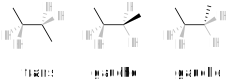
\includegraphics[width=0.5\textwidth]{\figpath/Model3_conformations.pdf}}
	
	As a result, the total number of conformations of a molecule with $n$ carbon-carbon bonds is $3^n$.

\end{model}

\begin{ctqs}

	\question How many possible conformations does the 700~kg/mol molecule of polyethylene considered earlier in this activity have?
	
		\begin{solution}[1in]
		\end{solution}
	
	\question 1~kg of 700~kg/mol polyethylene would contain approximately $9\times 10^{20}$ molecules.  Using this information, critique or defend the following statement in 2-3 complete sentences:
	
		\emph{``On average, a polymer sample will contain many molecules in each conformation.''}
	
		\begin{solution}[2.5in]
		\end{solution}
		
\end{ctqs}


\begin{exercises}

	\exercise In Model \ref{\labelbase:mdl:polyethyleneMW} (and the rest of this activity), we ignored the molecular weight of the end groups.  To determine whether or not this was a reasonable approximation, do the following:
	
		\begin{enumerate}
			
			\item Derive a formula for the molecular weight of a polyethylene molecule containing $N$ \ce{C2H4} repeat units and two \ce{CH3} end groups.
			
			\item Derive a formula for the molecular weight of a polyethylene molecule containing only $N$ \ce{C2H4} repeat units (i.e. without counting the end groups).
			
			\item Calculate the molecular weight obtained from each formula for $N=10$, $N=20$, $N=50$, $N=100$, $N=200$, and $N=500$. For each value of $N$, what is the percent error in the estimate obtained when you ignore the end groups, and above what degree of polymerization would you judge this error to be negligible?
			
		\end{enumerate}
		
	\exercise Summarize, in your own words, the key ways in which polymers differ from small molecules.
	
\end{exercises}


%\begin{problems}

%	\problem First exercise
%	\problem Second exercise
	
%\end{problems}


	
\end{activity}